\documentclass[resume]{subfiles}

\begin{document}
\section{Mémoire}
\begin{itemize}
\item Code ou texte
  \subitem Instructions binaires à être exécutée
  \subitem Elle est habituellement read-only
  \subitem Le Program Counter (PC) pointe sur la prochaine instruction à être exécutée
\item Données statiques: Variables globales/constantes/statiques partagées entre tâches/threads
\item Heap :Dynamique allouée avec malloc/free (C) ou new/delete (C++)
\item Stack
  \subitem Utilisé pour exécuter du code, méthode/fonction appel et retour
  \subitem Position est dans le stack Pointer
\end{itemize}

\subsection{Compiler Stages}
\begin{itemize}
\item Pre-processing
  \subitem Remplace les macros qui sont définie par un \# dans le code
  \subitem Fusionne les sous-fichiers (.c/.cpp, .h) en un seul fichier (remplace les includes .h par son texte interne)
\item Parser (analyseur)
  \subitem Lit le code C
  \subitem Vérifie les erreurs de syntaxes
  \subitem Créer un code intermédiaire (représentation en arbre)
\item Optimisateur Haut-niveau : modifie le code intermédiaire (indépendant du processeur)
\item Générateur de code (dès qu'on connait l'architecture)
  \subitem Crée le code assembleur étapes par étapes pour chaque noeud du code intermédiaire
  \subitem Alloue les registres à différentes utilisations
\item Optimisateur Bas-niveau : modifie le code assembleur (les parties sont spécifiques au processeur)
\item Linker/Loader : créer une image exécutable du fichier objet
\end{itemize}

\subsection{Model mémoire}
\begin{figure}[H]
    \centering
    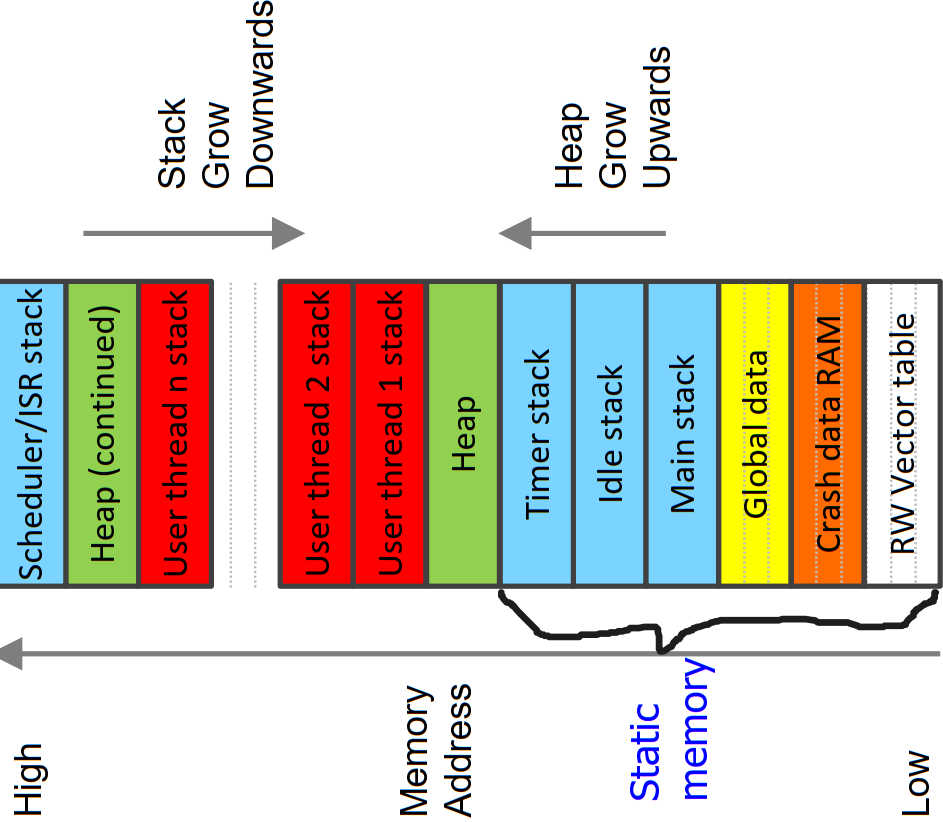
\includegraphics[width=0.6\columnwidth]{Figures/memoire/memoire.png}
\end{figure}

\subsection{Emplacement des données}
\begin{figure}[H]
    \centering
    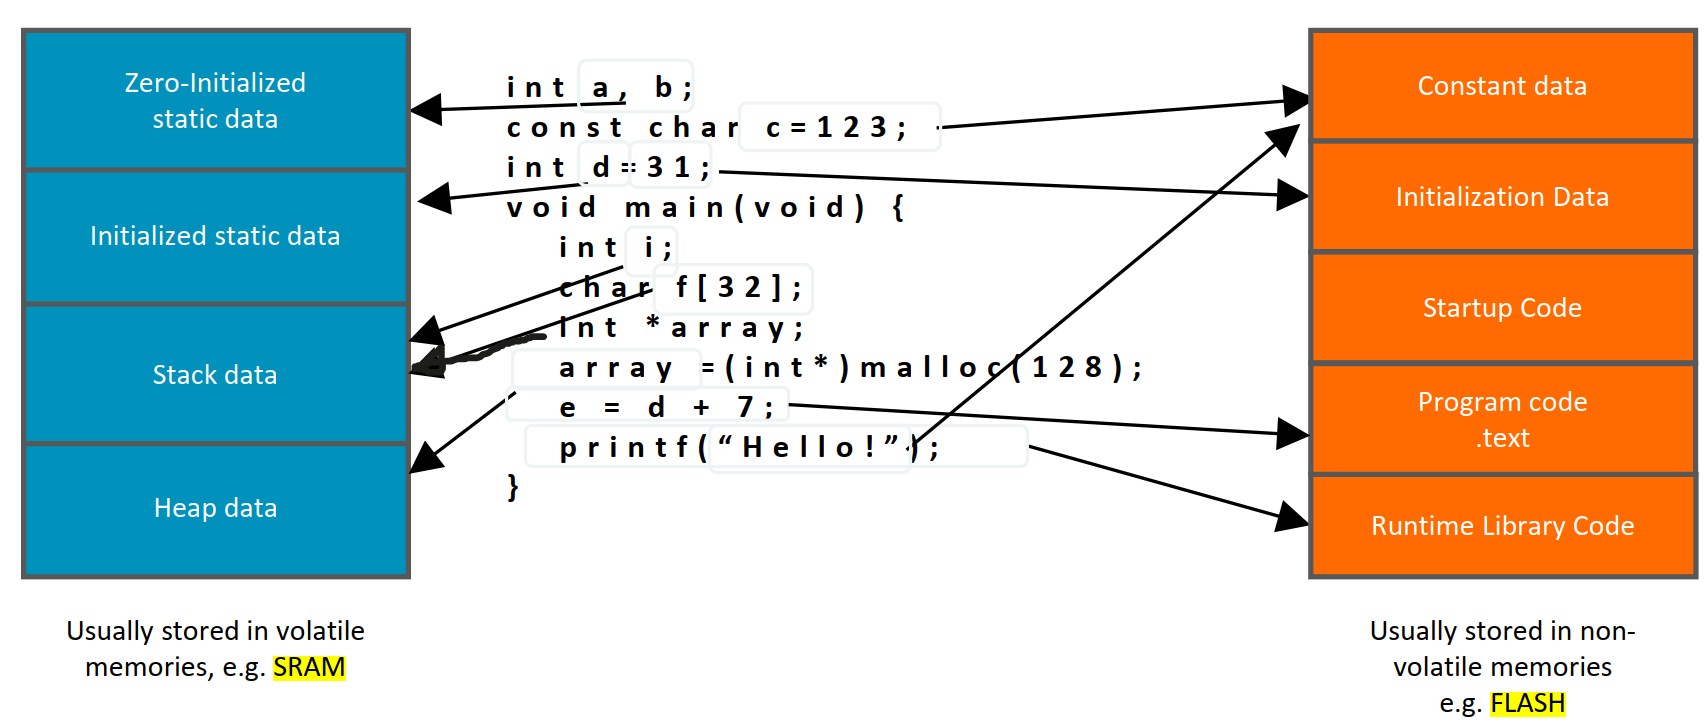
\includegraphics[width=0.6\columnwidth]{Figures/memoire/dataStorage.png}
\end{figure}

\subsection{Types de données}
\begin{itemize}
\item const : fixe en ROM
\item volatile : modifiable ISR pas d'optimisation
\item static : garde leurs valeurs entre deux appelles
\end{itemize}

\subsection{Hiérarchie mémoire (plus au moins rapide)}
\begin{itemize}
\item registres : dans le CPU
\item cache : (static RAM)
\item main memory : dynamic RAM, volatile data
\item secondary memory : flash/hard disk
\item tertiary memory : tape libraries
\end{itemize}

\subsection{Memory Protection Unit}

Améliore la sécurité peut définir 8 régions avec différents accès
\begin{itemize}
\item unité programmable
\item gère les accès mémoires et alloue des privilèges
\item monteur les transactions (data, instructions)
\item active un FAULT\_EXCEPTION lors d'une violation d'accès
\item (OS) définit régions mémoires
\item (OS) définit les permissions pour y accéder
\end{itemize}

\end{document}